\documentclass[14pt]{beamer}

\usetheme{Montpellier}
\usecolortheme{beaver}

\usepackage{amsmath, amssymb, ../../vimacros, hyperref, tikz, subcaption}
\usepackage{physics}
\usetikzlibrary{positioning, fit, bayesnet, shapes.misc, patterns}
\usepackage[round]{natbib}

\beamertemplatenavigationsymbolsempty

\hypersetup{breaklinks=true, colorlinks=true, linkcolor=blue, urlcolor=blue, citecolor=blue}

\pgfdeclarepatternformonly{stripes}
{\pgfpointorigin}{\pgfpoint{.4cm}{.4cm}}
{\pgfpoint{.4cm}{.4cm}}
{
	\pgfpathmoveto{\pgfpoint{0cm}{0cm}}
	\pgfpathlineto{\pgfpoint{.4cm}{.4cm}}
	\pgfpathlineto{\pgfpoint{.4cm}{.2cm}}
	\pgfpathlineto{\pgfpoint{.2cm}{0cm}}
	\pgfpathclose
	\pgfusepath{fill}
	\pgfpathmoveto{\pgfpoint{0cm}{0.2cm}}
	\pgfpathlineto{\pgfpoint{0cm}{.4cm}}
	\pgfpathlineto{\pgfpoint{0.2cm}{.4cm}}
	\pgfpathclose
	\pgfusepath{fill}
}

\title{Normalising Flows}
\author{Philip Schulz and Wilker Aziz\\
\url{https://github.com/philschulz/VITutorial}}
\date{}

\setbeamertemplate{footline}[frame number]

\begin{document}

\begin{frame}
\maketitle
\end{frame}

\begin{frame}
\tableofcontents
\end{frame}

\section{The problem with Known Distributions}

\begin{frame}
\tableofcontents[current]
\end{frame}

\begin{frame}{The Case of Pictures}
Have you modeled pixels as Gaussian variables?
Do we really believe that the pixels follow a Gaussian distribution?
\begin{figure}
\begin{subfigure}{.3\textwidth}

\includegraphics[scale=.02]{cat1.jpg} 
\end{subfigure}
~
\begin{subfigure}{.3\textwidth}
\includegraphics[scale=.02]{cat2.jpg} 
\end{subfigure}
~
\begin{subfigure}{.3\textwidth}
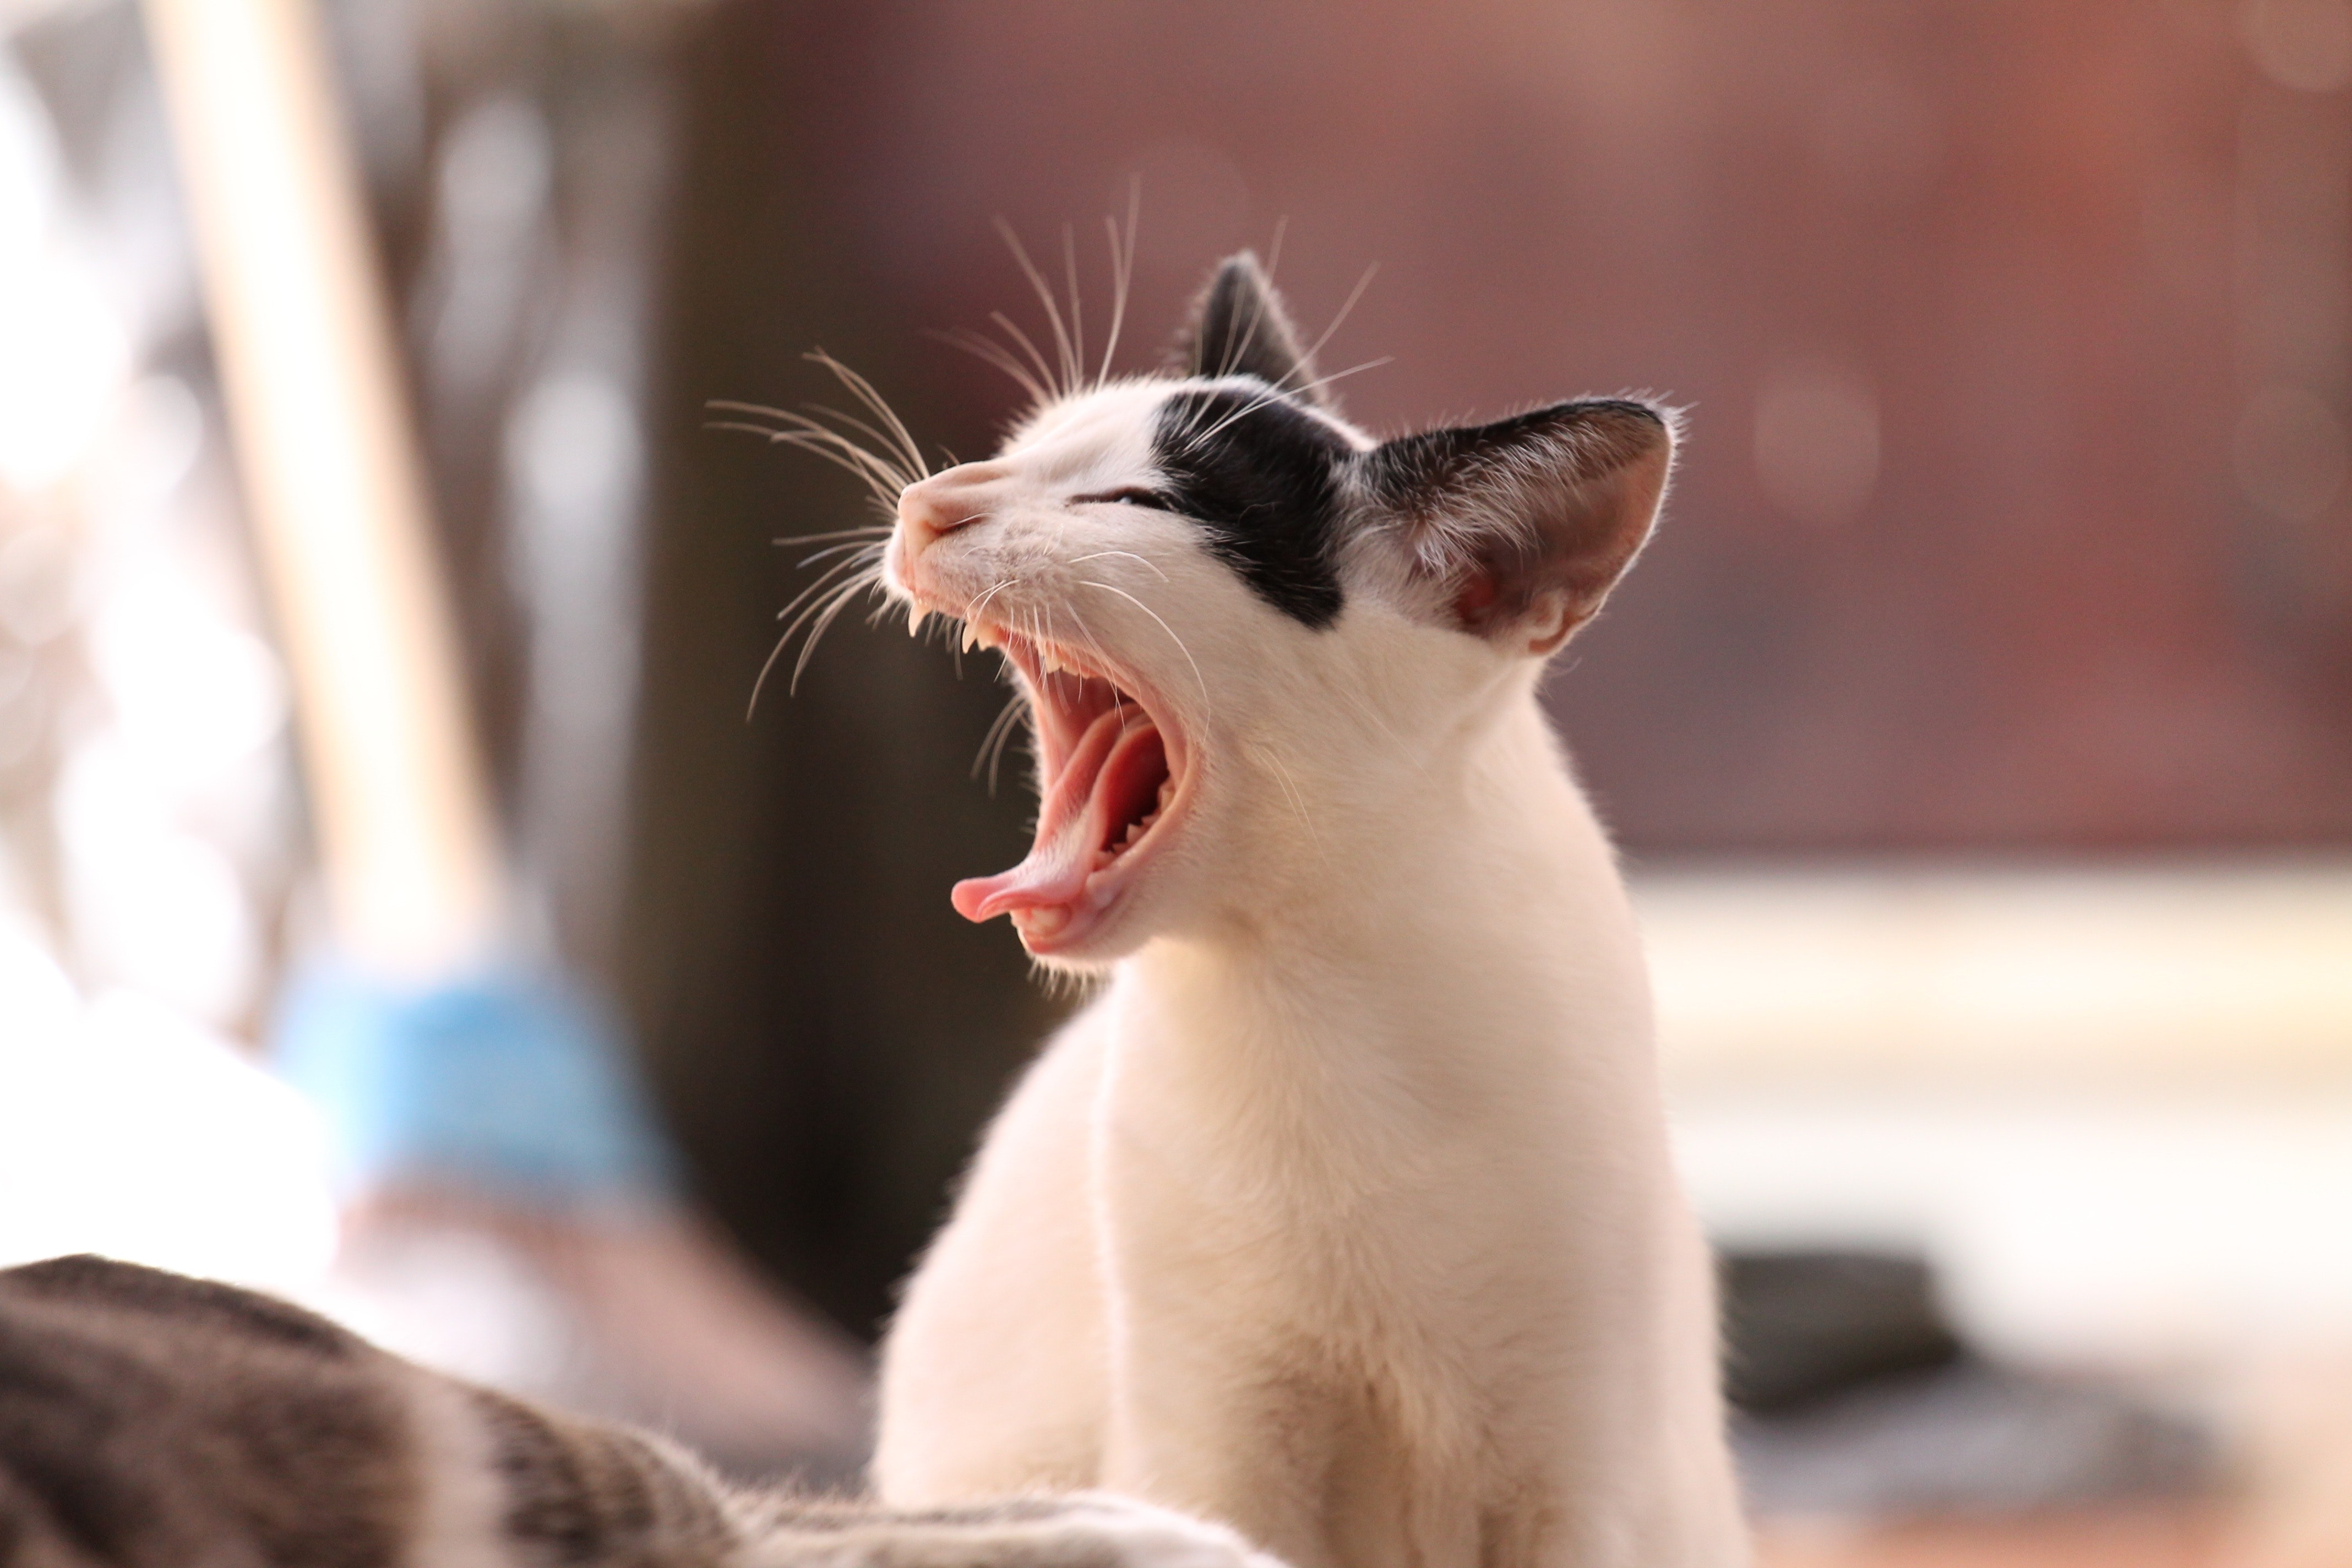
\includegraphics[scale=.02]{cat3.jpg} 
\end{subfigure}
\end{figure}
\end{frame}

\begin{frame}{The case of Word Embeddings}
\pause
\begin{figure}
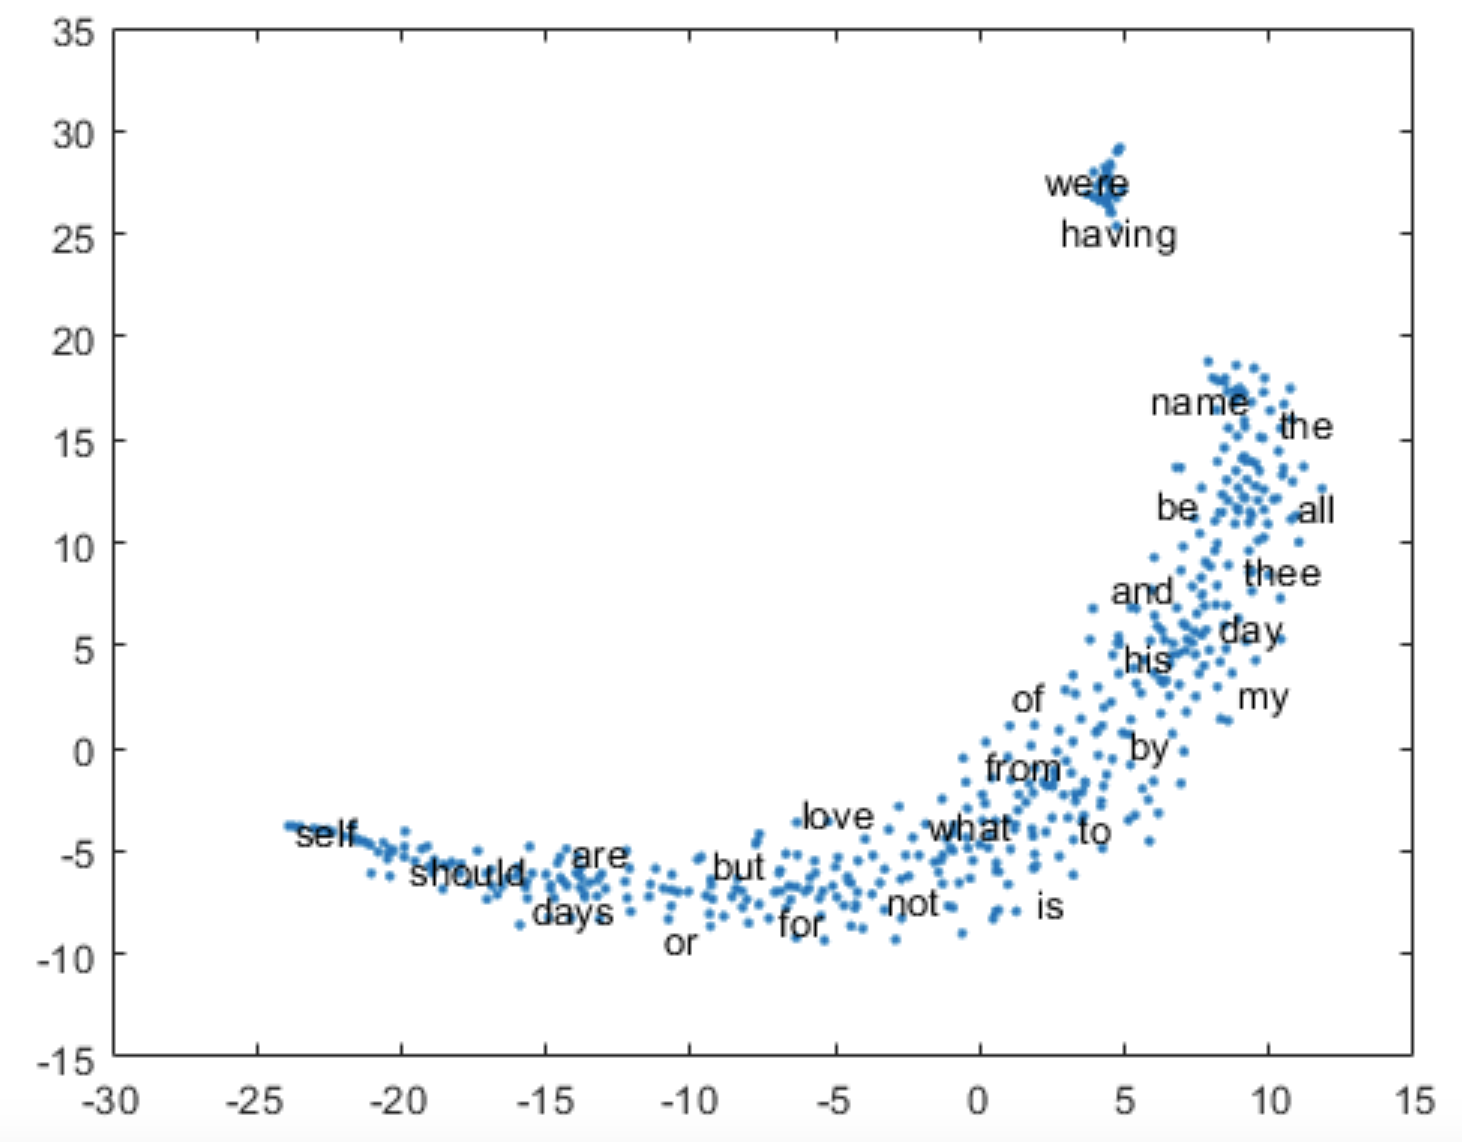
\includegraphics[scale=.2]{wordcloud.png}
\caption{\url{https://it.mathworks.com/help/textanalytics/ref/trainwordembedding.html}}
\end{figure}
\end{frame}

\begin{frame}{Posterior Approximations}
We often use exponential families to approximate posteriors. Thus we assume unimodal posteriors. Is that realistic?
\pause
\begin{block}{Counter example}
Gaussian mixture model
\end{block}
\end{frame}

\section{Normalising Flows}

\begin{frame}
\tableofcontents[current]
\end{frame}

\begin{frame}{Recap: Reparametrisation}
Express the density of a variable $ Y $ in terms of the density of a variable $ X $. Assume that a differentiable, invertible mapping
$ h: \mathcal{X} \rightarrow \mathcal{Y} $ exists.
\begin{equation*}
\begin{aligned}
h(x) &= y \\ \pause
p_{Y}(y) &= p_{X}(h^{-1}(y))\djac{h^{-1}}{y} = p(x)\djac{h^{-1}}{y}  \\ \pause
p_{X}(x) &= p_{Y}(h(x))\djac{h}{x} = p(y)\djac{h}{x}
\end{aligned}
\end{equation*}
\pause
\begin{block}{The Challenge}
The mapping $ h $ (or its inverse) needs to be defined.
\end{block}
\end{frame}

\begin{frame}{Normalising Flows}
\begin{block}{Approach}
Let's learn the transformation $ h $ (or its inverse).
\end{block}
\pause
\begin{block}{Problem}
If we want $ p(y) $, we need to provide $ \djac{h^{-1}}{y} $ \textbf{in the forward pass}. But that's hard!
\end{block}
We are going to devise ways to get $ \djac{h^{-1}}{y} $.
\end{frame}

\begin{frame}{Normalising Flows}
\begin{block}{Core Idea}
Decompose mapping $ h: \mathcal{X} \rightarrow \mathcal{Y} $ into 
\begin{equation*}
h = h_{1}\circ h_{2}\circ\ldots\circ h_K \ .
\end{equation*}
\pause
Now we can learn $ K $ mappings with simple jacobian determinants.
\begin{small}
\pause
\begin{equation*}
\begin{aligned}
h^{-1} &= h_{K}^{-1}\circ h_{K-1}^{-1} \circ \ldots \circ h_{1}^{-1} \\ \pause
p_{X}(x) &= p_{Y}(y) \djac{h_{1}}{y^{(1)}}\djac{h_{2}}{y^{(2)}}\ldots \djac{h_{K}}{x} \\ \pause
p_{Y}(y) &= p_{X}(x)\djac{h_{1}^{-1}}{y^{(K-1)}} \djac{h_{2}^{-1}}{y^{(K-2)}}\ldots \djac{h_{1}^{-1}}{y}
\end{aligned}
\end{equation*}
\end{small}
\end{block}
\end{frame}

\begin{frame}{Normalising Flows}
\begin{figure}
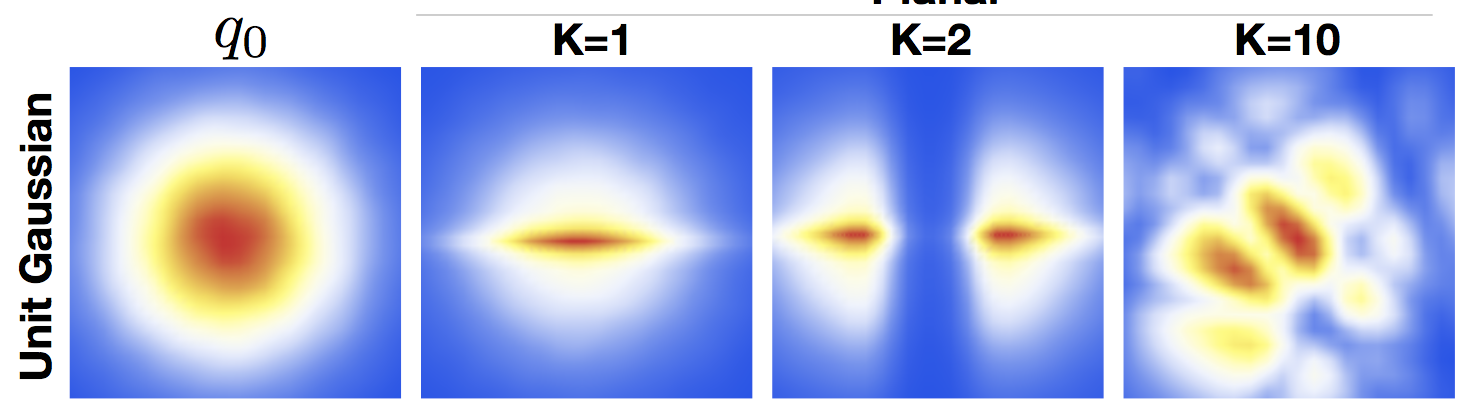
\includegraphics[scale=.4]{nf.png}
\caption{Taken from \cite{RezendeMohamed:2015}}
\end{figure}
\end{frame}

\section{Use Case 1: Density Estimation}
\begin{frame}
\tableofcontents[current]
\end{frame}

\begin{frame}{Normalising Flows: Density Estimation}
\begin{block}{Setting}
Our data $ x $ is has unknown continuous density $ p(x) $.
We can therefore not handcraft a likelihood.
\end{block}
\pause
\begin{block}{Goal}
Transform known variable $ x $ into $ \epsilon = h(x) $ with \textbf{known} density $ p_{\epsilon}(\epsilon) $ and express the likelihood as
\begin{small}
\pause
\begin{equation*}
\begin{aligned}
p_{X}(x) &= p_{\epsilon}(\epsilon)\djac{h}{x} \\ \pause
&= p_{\epsilon}(\textcolor{blue}{\epsilon})\djac{h_{1}}{\epsilon^{(1)}}\djac{h_{2}}{\epsilon^{(2)}}\ldots \djac{h_{K}}{x} \\ \pause
&= p_{\epsilon}(\textcolor{blue}{h_{1}(\epsilon^{(1)})})\djac{h_{1}}{\epsilon^{(1)}}\ldots \djac{h_{K}}{x}
\end{aligned}
\end{equation*}
\end{small}
\end{block}
\end{frame}

\begin{frame}{2-step Flow}
\begin{equation*}
\begin{aligned}
p_{X}(x) &= p_{\epsilon}(\textcolor{blue}{\epsilon})\djac{h_{1}^{-1}}{\textcolor{red}{\epsilon^{(1)}}}\djac{h_{2}^{-1}}{x} \\ \pause
&= p_{\epsilon}(\textcolor{blue}{h_{1}^{-1}(h_{2}^{-1}(x))})\djac{h_{1}^{-1}}{\textcolor{red}{h_{2}^{-1}(x)}}\djac{h_{2}^{-1}}{x}
\end{aligned}
\end{equation*}
\pause
The transformations $ h^{-1}_{1} $ and $ h^{-1}_{2} $ are learned by backprop. The determinants need to be computed analytically.
\end{frame}

\begin{frame}{Designing a Transformation}
Assume: $ x = (x_{1}, x_{2}, \ldots x_{M}) $.
Then factorise the density according to the chain rule.
\begin{equation*}
\log p(x|\theta) = \sum_{j=1}^{M} \log p(x_{j}|x_{<j}\theta)
\end{equation*}
Next assume an invertible mapping $ h(x_{j}) = \epsilon_{j} $.
\begin{block}{Simple Mapping}
\begin{equation*}
\begin{aligned}
h(x) &= \epsilon \\
h^{-1}(\epsilon) &= x
\end{aligned}
\end{equation*}
\end{block}
\end{frame}

\begin{frame}{Designing a Transformation}
Assume: $ x = (x_{1}, x_{2}, \ldots x_{M}) $.
Then factorise the density according to the chain rule.
\begin{equation*}
\log p(x|\theta) = \sum_{j=1}^{M} \log p(x_{j}|x_{<j}\theta)
\end{equation*}
Next assume a mapping $ h(x_{j}) = \epsilon_{j} $.
\begin{block}{Flow Mapping}
\begin{equation*}
\begin{aligned}
h_{1}\circ h_{2} \circ\ldots\circ h_{K}(x) &= \epsilon \\
h^{-1}_{K}\circ h^{-1}_{K-1}\circ\ldots \circ h^{-1}_{1}(\epsilon) &= x
\end{aligned}
\end{equation*}
\end{block}
\end{frame}

\begin{frame}{Designing a Transformation}
\begin{block}{MADE \citep{GermainEtAl:2015}}
An autoregressive network that takes constant time. Its connectivity matrix is lower-triangular.
\begin{equation*}
\begin{bmatrix}
0 & 0 & \cdots & 0 & 0 \\
1 & 0 & \cdots & 0 & 0 \\
1 & 1 & \cdots & 0 & 0 \\
\vdots & \vdots & \cdots & \vdots & \vdots \\
1 & 1 & \cdots & 1 & 0
\end{bmatrix}
\end{equation*}
\end{block}
\end{frame}

\begin{frame}{Designing a Transformation}
\begin{figure}
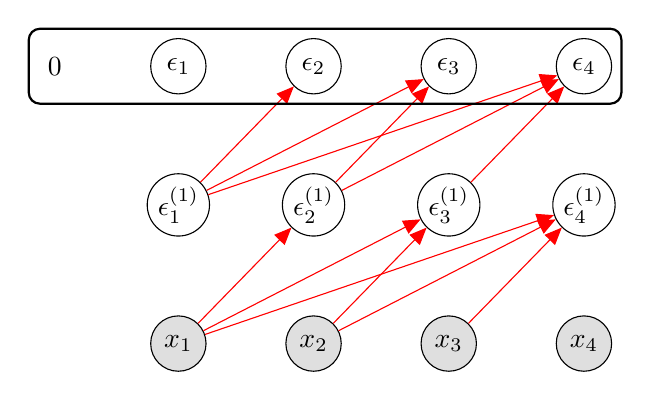
\begin{tikzpicture}
\node[obs] (x1) {$x_{1}$};
\node[obs, right = of x1] (x2) {$x_{2}$};
\node[obs, right = of x2] (x3) {$x_{3}$};
\node[obs, right = of x3] (x4) {$x_{4}$};

\pause

\node[latent, above = of x1] (e11) {$\epsilon^{(1)}_{1}$};
\node[latent, above = of x2] (e12) {$\epsilon^{(1)}_{2}$};
\node[latent, above = of x3] (e13) {$\epsilon^{(1)}_{3}$};
\node[latent, above = of x4] (e14) {$\epsilon^{(1)}_{4}$};

\edge[color=red]{x1}{e12};
\edge[color=red]{x1,x2}{e13};
\edge[color=red]{x1,x2,x3}{e14};

\pause

\node[latent, above = of e11] (e21) {$\epsilon_{1}$};
\node[latent, above = of e12] (e22) {$\epsilon_{2}$};
\node[latent, above = of e13] (e23) {$\epsilon_{3}$};
\node[latent, above = of e14] (e24) {$\epsilon_{4}$};

\edge[color=red]{e11}{e22};
\edge[color=red]{e11,e12}{e23};
\edge[color=red]{e11,e12,e13}{e24};

\pause

\node[left = of e21] (n1) {$\NDist{0}{\IMatrix}$};
\node[draw=black, thick, rectangle, fit= (n1)(e21)(e22)(e23)(e24), rounded corners] {};
\end{tikzpicture}
\end{figure}
\end{frame}

\begin{frame}{Designing a Transformation}
We use a MADE $ g^{(2)}_{\theta} $ to predict the parameters of the first transformation: $ \begin{bmatrix} \mu_{j} & \sigma_{j} \end{bmatrix} =  g^{(2)}_{\theta}(x_{<j}) $.
Then we apply the first transformation.
\begin{equation*}
\begin{aligned}
\epsilon_{j}^{(1)} &= h_{2}^{-1}(x)_{j} &= \frac{x_{j} - \mu(x_{<j})}{\sigma(x_{<j})} \\ \pause
\epsilon^{(1)} &= h_{2}^{-1}(x) &= \frac{x - \mu}{\sigma}
\end{aligned}
\end{equation*}
\pause
The Jacobian is
\begin{equation*}
\jac{h_{2}^{-1}}{x} = \pause \IMatrix\sigma^{-1} + J_{\frac{-\mu}{\sigma}}(x)
\end{equation*}
\end{frame}

\begin{frame}{Designing a Transformation}
Define $ \alpha_{lj} = \frac{d}{dx_{l}}\frac{-\mu_{j}}{\sigma_{j}} $.
\begin{small}
\begin{equation*}
\begin{aligned}
&\jac{h_{K}^{-1}}{x} = \IMatrix\sigma^{-1} + J_{\frac{-\mu}{\sigma}}(x) = \\ \pause
&\begin{bmatrix}
\sigma^{-1}_{11} & 0 & \cdots & 0 & 0 \\
0 & \sigma^{-1}_{22} & \cdots & 0 & 0 \\
0 & 0 & \cdots & 0 & 0 \\
\vdots & \vdots & \cdots & \vdots & \vdots \\
0 & 0 & \cdots & 0 & \sigma^{-1}_{mm}
\end{bmatrix}
\pause
+
\begin{bmatrix}
0 & 0 & \cdots & 0 & 0 \\
\alpha_{21} & 0 & \cdots & 0 & 0 \\
\alpha_{31} & \alpha_{32} & \cdots & 0 & 0 \\
\vdots & \vdots & \cdots & \vdots & \vdots \\
\alpha_{m1} & \alpha_{m2} & \cdots & \alpha_{m,m-1} & 0
\end{bmatrix}
\end{aligned}
\end{equation*}
\end{small}
\end{frame}

\begin{frame}{Designing a Transformation}
\begin{block}{Simple Jacobian Determinant}
\begin{equation*}
\djac{h_{2}^{-1}}{x} = \prod_{j=1}^{M}\sigma^{-1}_{j}
\end{equation*}
\pause
In practice we work with the log-likelihood.
\begin{equation*}
\log\djac{h_{2}^{-1}}{x} = -\sum_{j=1}^{M}\log\sigma_{j}
\end{equation*}
\end{block}
\end{frame}

\begin{frame}{2-step Flow}
\begin{small}
\begin{equation*}
\begin{aligned}
p_{X}(x) &= p_{\epsilon}(\textcolor{blue}{\epsilon})\djac{h_{1}^{-1}}{\textcolor{red}{\epsilon^{(1)}}}\djac{h_{2}^{-1}}{x} \\
&= p_{\epsilon}(\textcolor{blue}{h_{1}^{-1}(h_{2}^{-1}(x))})\djac{h_{1}^{-1}}{\textcolor{red}{h_{2}^{-1}(x)}}\djac{h_{2}^{-1}}{x} \\ \pause
\log p_{X}(x) &= \log p_{\epsilon}(\textcolor{blue}{h_{1}^{-1}(h_{2}^{-1}(x))})\pause -\sum_{j=1}^{M}\log\sigma^{(2)}_{j}-\sum_{j=1}^{M}\log\sigma^{(1)}_{j}
\end{aligned}
\end{equation*}
\end{small}
\pause
\begin{equation*}
\begin{aligned}
\epsilon^{(1)} = h^{-1}_{2} = \frac{x - \mu^{(2)}}{\sigma^{(2)}} \text{ where } \begin{bmatrix}\mu^{(2)}, \sigma^{(2)}\end{bmatrix} = g^{(2)}(x) \\ \pause
\epsilon = h^{-1}_{1} = \frac{\epsilon^{(1)} - \mu^{(1)}}{\sigma^{(1)}} \text{ where } \begin{bmatrix}\mu^{(1)}, \sigma^{(1)}\end{bmatrix} = g^{(1)}(\epsilon^{(1)})
\end{aligned}
\end{equation*}
\end{frame}

\begin{frame}{Intermediate Summary}
\begin{itemize}
\item NFs map transform complex distributions to simpler ones (or vice versa)
\item Use in density estimation for complex distributions
\item Jacobian needs to be carefully designed
\item Sampling is slow because sequential
\end{itemize}
\end{frame}

\section{Use Case 2: Inference (sampling)}
\begin{frame}
\tableofcontents[current]
\end{frame}

\begin{frame}{Setting}
We have a generative model $ p(x|z) $. We want to approximate the posterior $ p(z|x) $ using an amortized variational distribution $ q(z|x) $ computed by a neural net.
\pause
\begin{block}{Goal}
We want a complex, multimodal approximate posterior $ q(z|x) $.
\end{block}
\end{frame}

\begin{frame}{Normalising Flows: Inference}
\begin{equation*}
\begin{aligned}
\ELBO &= -\KL{q(z|x)}{p(z|x)} \\
&= \E[q(z|\lambda)]{\log p(x|z)} - \KL{q(z|\lambda))}{p(z)} \\
&= \underbrace{\E[q(\epsilon)]{\log p(x|h^{-1}(\epsilon))}}_{\text{sample $ z $}} - \underbrace{\KL{q(z|\lambda)}{p(z)}}_{\text{assess density}}
\end{aligned}
\end{equation*}
\begin{block}{Simple Mapping}
\begin{equation*}
\begin{aligned}
h(z) &= \epsilon \text{ s.t. } \epsilon \perp \lambda \\
h^{-1}(\epsilon) &= z = z^{(K)}
\end{aligned}
\end{equation*}
\end{block}
\end{frame}

\begin{frame}{Normalising Flows: Inference}
\begin{equation*}
\begin{aligned}
&-\KL{q(z|x)}{p(z|x)} \propto \ELBO = \\
&= \E[q(z|\lambda)]{\log p(x|z)} - \KL{q(z|\lambda))}{p(z)} \\
&= \underbrace{\E[q(\epsilon)]{\log p(x|h^{-1}(\epsilon))}}_{\text{sample $ z $}} - \underbrace{\KL{q(z|\lambda)}{p(z)}}_{\text{assess density}}
\end{aligned}
\end{equation*}
\begin{block}{Flow Mapping}
\begin{equation*}
\begin{aligned}
h_{1}\circ h_{2}\circ \ldots \circ h_{K}(z) &= \epsilon \text{ s.t. } \epsilon \perp \lambda \\
h^{-1}_{K}\circ h^{-1}_{K-1}\circ\ldots \circ h^{-1}_{1}(\epsilon) &= z
\end{aligned}
\end{equation*}
\end{block}
\end{frame}

\begin{frame}{2-step Flow}
\begin{small}
\begin{equation*}
\begin{aligned}
q_{Z}(z^{(2)}) &= q_{\epsilon}(\epsilon)\djac{h_{1}}{\textcolor{red}{z^{(1)}}}\djac{h_{2}}{\textcolor{blue}{z^{(2)}}} \\ \pause
&= q_{\epsilon}(\epsilon)\djac{h_{1}}{\textcolor{red}{h_{1}(\epsilon)}}\djac{h_{2}}{\textcolor{blue}{h_{2}(h_{1}(\epsilon))}}
\end{aligned}
\end{equation*}
\end{small}
\pause
The transformations $ h_{1} $ and $ h_{2} $ are learned by backprop. The determinants need to be computed analytically.
\end{frame}

\begin{frame}{Designing a Transformation}
We are again going to use a MADE to predict parameters. However, this time we will use it in the other direction.
\end{frame}

\begin{frame}{Designing a Transformation}
\begin{figure}
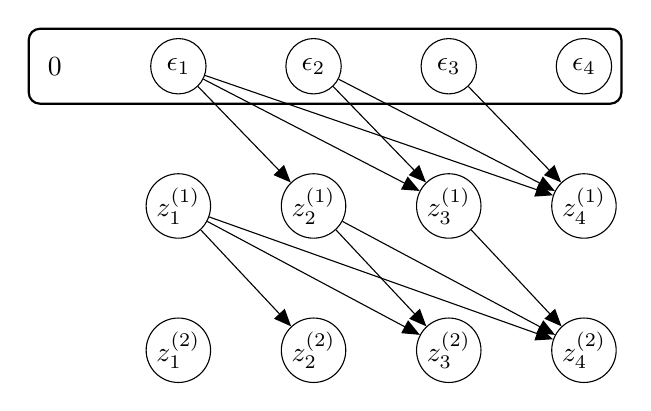
\begin{tikzpicture}
\node[latent] (e1) {$\epsilon_{1}$};
\node[latent, right = of e1] (e2) {$\epsilon_{2}$};
\node[latent, right = of e2] (e3) {$\epsilon_{3}$};
\node[latent, right = of e3] (e4) {$\epsilon_{4}$};

\node[left = of e1] (n1) {$\NDist{0}{\IMatrix}$};
\node[draw=black, thick, rectangle, fit= (n1)(e1)(e2)(e3)(e4), rounded corners] {};

\pause

\node[latent, below = of e1] (z11) {$z^{(1)}_{1}$};
\node[latent, below = of e2] (z12) {$z^{(1)}_{2}$};
\node[latent, below = of e3] (z13) {$z^{(1)}_{3}$};
\node[latent, below = of e4] (z14) {$z^{(1)}_{4}$};

\edge{e1}{z12,z13,z14};
\edge{e2}{z13,z14};
\edge{e3}{z14};

\pause

\node[latent, below = of z11] (z21) {$z^{(2)}_{1}$};
\node[latent, below = of z12] (z22) {$z^{(2)}_{2}$};
\node[latent, below = of z13] (z23) {$z^{(2)}_{3}$};
\node[latent, below = of z14] (z24) {$z^{(2)}_{4}$};

\edge{z11}{z22,z23,z24};
\edge{z12}{z23,z24};
\edge{z13}{z24};
\end{tikzpicture}
\end{figure}
\end{frame}

\begin{frame}{Designing a Transformation}
We use a MADE $ f_{\lambda} $ to predict the parameters of the first transformation: $ \begin{bmatrix} \mu_{j} & \sigma_{j} \end{bmatrix} =  f_{\lambda}(\epsilon_{<j}) $.
Then we apply the first transformation.
\begin{equation*}
\begin{aligned}
z^{(1)}_{j} &= h_{1}(\epsilon)_{j} &= \mu(\epsilon_{<j}) + \sigma(\epsilon_{<j}) \epsilon_{j} \\ \pause
z^{(1)} &= h_{1}(\epsilon) &= \mu + \sigma \epsilon
\end{aligned}
\end{equation*}
\pause
\begin{equation*}
\jac{h_{1}}{\epsilon} = \IMatrix \sigma + \jac{\mu}{\epsilon} +\jac{\sigma \epsilon}{\epsilon}
\end{equation*}
\end{frame}

\begin{frame}{Designing a Transformation}
\begin{block}{Simple Jacobian Determinant}
\begin{equation*}
\djac{h_{1}}{\epsilon} = \prod_{j=1}^{M}\sigma_{j}
\end{equation*}
In practice we work with the log-likelihood.
\begin{equation*}
\log\djac{h_{1}}{\epsilon} = \sum_{j=1}^{M}\log\sigma_{j}
\end{equation*}
\end{block}
\end{frame}

\begin{frame}{2-step Flow}
\begin{small}
\begin{equation*}
\begin{aligned}
q_{Z}(z^{(2)}) &= q_{\epsilon}(\epsilon)\djac{h_{1}}{\textcolor{red}{z^{(1)}}}\djac{h_{2}}{\textcolor{blue}{z^{(2)}}} \\
&= q_{\epsilon}(\epsilon)\djac{h_{1}}{\textcolor{red}{h_{1}(\epsilon)}}\djac{h_{2}}{\textcolor{blue}{h_{2}(h_{1}(\epsilon))}} \\ \pause
\log q_{Z}(z^{(2)}) &= \log q_{\epsilon}(\epsilon) \pause + \sum_{j=1}^{M}\log\sigma^{(1)}_{j} + \sum_{j=1}^{M}\log\sigma^{(2)}_{j}
\end{aligned}
\end{equation*}
\end{small}
\pause
\begin{equation*}
\begin{aligned}
z^{(1)} &= \mu^{(1)} + \sigma^{(1)}\epsilon \text{ where } \begin{bmatrix}\mu^{(1)}, \sigma^{(1)}\end{bmatrix} = f^{(1)}_{\lambda}(\epsilon) \\ \pause
z^{(2)} &= \mu^{(2)} + \sigma^{(2)}z^{(1)} \text{ where } \begin{bmatrix}\mu^{(2)}, \sigma^{(2)}\end{bmatrix} = f^{(2)}_{\lambda}(z^{(1)})
\end{aligned}
\end{equation*}
\end{frame}

\begin{frame}{ELBO}
Recall: $ z = z^{(2)} $
\begin{small}
\begin{equation*}
\begin{aligned}
&\ELBO = \E[q(z|\lambda)]{\log p(x|z)} - \KL{\textcolor{blue}{q(z)|\lambda))}}{p(z)} = \\ \pause
&\E[q(z|\lambda)]{\log p(x|z)} - \KL{\textcolor{blue}{q(\epsilon)\djac{h}{z}}}{p(z)}
\end{aligned}
\end{equation*}
\end{small}
\end{frame}

\begin{frame}{ELBO}
\begin{small}
\begin{block}{KL-term}
\begin{equation*}
\begin{aligned}
&\KL{q(\epsilon)\djac{h}{z}}{p(z)} = \\ \pause
&\E[q(z|\lambda))]{\log\frac{q(\epsilon)\djac{h}{z}}{p(z)}} \pause \overset{\text{MC}}{\approx} \frac{1}{S}\sum_{s=1}^{S} \log\frac{q(\epsilon)\djac{h}{z^{(s)}}}{p(z^{(s)})}
\end{aligned}
\end{equation*}
\end{block}
\pause
\begin{block}{Jacobian}
\pause
\begin{equation*}
\djac{h}{z^{(s)}} = \sum_{j=1}^{M}\log\sigma^{(1)}_{j} + \sum_{j=1}^{M}\log\sigma^{(2)}_{j}
\end{equation*}
\end{block}
\end{small}
\end{frame}

%\begin{frame}{Other Appliations of Normalizing Flows}
%\begin{itemize}
%\item As a prior
%\pause
%\item Modeling of dynamic systems
%\end{itemize}
%\end{frame}

\section{Summary}

\begin{frame}{Summary}
\begin{itemize}
\item NFs model arbitrary continuous distributions
\item They allow for density computation
\item Need to have simple Jacobian determinants
\item Depending on direction, they are good at either sampling or density computation (not both)
\end{itemize}
\end{frame}

\begin{frame}[allowframebreaks]{References}
\bibliographystyle{plainnat}
\bibliography{../../VI}
\nocite{KingmaEtAl:2016, RezendeMohamed:2015, HuangEtAl:2018}
\end{frame}

\end{document}